\documentclass[12pt, a4paper, twoside]{article}
\usepackage[utf8]{inputenc}
\usepackage[cm]{fullpage}
\usepackage{fancyhdr}
\usepackage{textcomp}
\usepackage{graphicx}
\usepackage{commath}
\usepackage[portuguese]{babel}

\begin{document}

\title{Pré-relatório 3 do Laboratório de Dispositivos e Circuitos Eletrônicos}
\author{Cristiano Silva Júnior: 13/0070629}
\date{\today}
\maketitle

Neste relatório, vamos utilizar três modelos para o diodo. O primeiro deles é o modelo
ideal, em que o diodo é um circuito fechado para quedas de tensão positivas e um
circuito aberto para quedas de tensão negativas.

% TODO Add image for diode model.

O segundo modelo a ser utilizado é o modelo de queda de tensão constante, em que o
diodo passa a ser um diodo ideal com uma fonte de tensão em série. Neste caso, o diodo
somente conduz para tensões maiores do que a sua tensão de polarização.

% TODO Add image for constant tension diode model.

Neste modelo, podemos levar em conta o efeito Zener, em que, para alguns diodos, o diodo
também conduz para quedas de tensão muito negativas. No caso, um diodo com
características de Zener conduz também para tensões menores que a sua tensão de Zener.

O terceiro modelo é o chamado diodo real, em que a corrente $i$ que passa pelo diodo
depende da tensão $V$ aplicada sobre ele:
$$i = I_s\left( e^{\frac{V}{nV_T}} - 1 \right)$$

\section{Exercício 1}

% TODO Add image describing circuit to be solved.

Para resolver o exercício proposto, vamos utilizar o modelo do diodo ideal. Neste caso,
a saida do circuito é trivial e é descrita na figura 4 para uma entrada unitária.

\begin{figure}
    \centering
    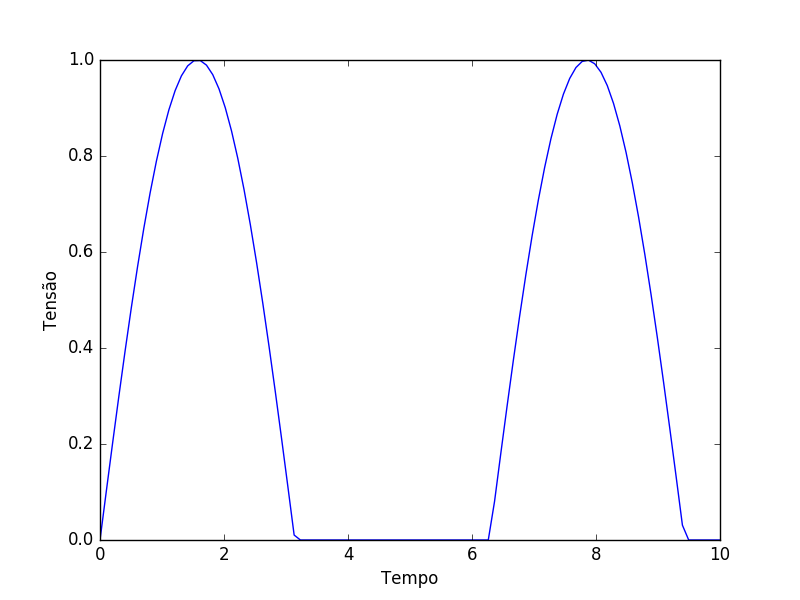
\includegraphics[width=0.8\textwidth]{figs/rel3/ex1.png}
    \caption{Saída do circuito do problema 1}
\end{figure}

\section{Exercício 2}

Utilizando o modelo do diodo ideal, nota-se que
\begin{equation}
    v_o(t) =
    \begin{cases}
        v_i(t), & \text{se}\ v_i(t) > 0 \\
        0, & \text{caso contrário}
    \end{cases}
\end{equation}

Sendo assim, a característica de transferência do circuito será como o descrito na
figura 5.

\begin{figure}
    \centering
    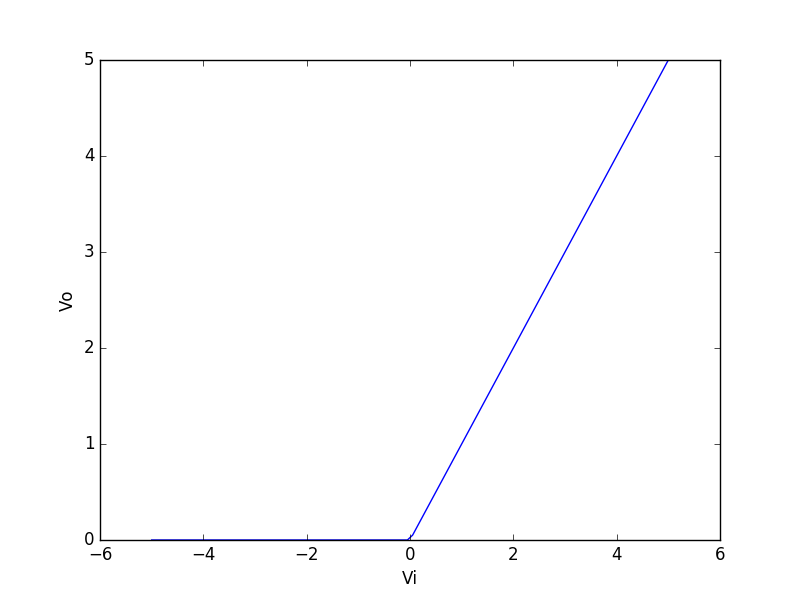
\includegraphics[width=0.8\textwidth]{figs/rel3/ex2.png}
    \caption{Característica de transferência do circuito dos problemas 1 e 2}
\end{figure}

\section{Exercício 3}

Segundo Schroen, o modelo que é utilizado nesta disciplina para o diodo obedece a
chamada equação de Shockley para o diodo:
$$i = I_s\left( e^{\frac{V}{nV_T}} - 1 \right)$$
onde $I_s$ é a corrente de saturação;
$V_D$, a tensão sobre o diodo;
$V_T$, a tensãotérmica; e
$n$, o fator de idealidade do diodo (geralmente igual a 1 ou 2 para diodos
de silício).

\section{Exercício 4}

Pelo \textit{datasheet} da \textit{Fairchild Instruments}, a tensão de polarização
do \textit{1N4007} é $V_F = 1.1V$ para correntes iguais a $1A$.

\section{Exercício 5}

% TODO Add diagram for circuit 2.a

Utilizando o modelo de queda de tensão constante, é fácil ver que a característica
de transferência do circuito será
\begin{equation}
    v_s(t) =
    \begin{cases}
        V - V_F & \forall\ V \geq V_F \\
        0, & \text{caso contrário}
    \end{cases}
\end{equation}

Neste caso,
\begin{figure}
    \centering
    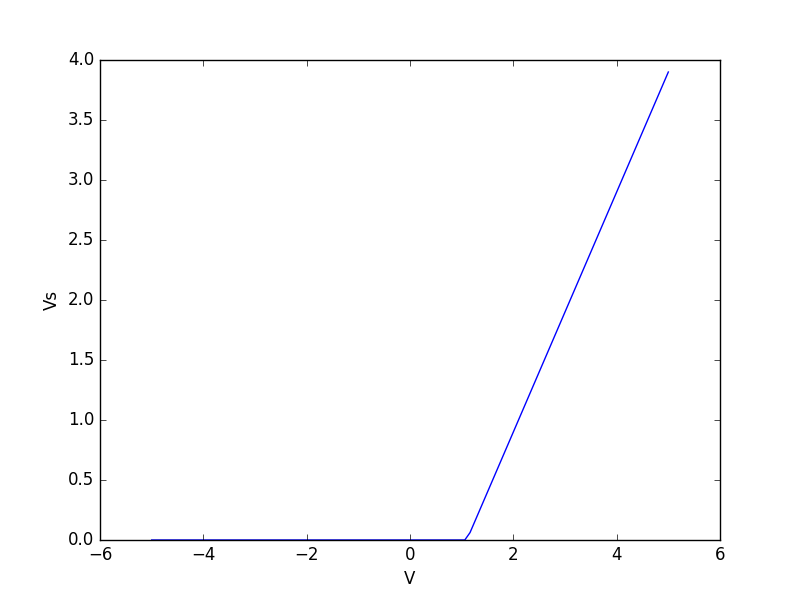
\includegraphics[width=0.8\textwidth]{figs/rel3/ex5.png}
    \caption{Curva da característica de transferência do sistema do problema 5}
\end{figure}

\section{Exercício 6}

Para analisar o circuito, vamos analisar inicialmente o semiciclo positivo e depois
o negativo. Para o positivo, o circuito equivalente é o da figura X.

% TODO Add image for the direct wave circuit

Neste caso,
\begin{equation}
    v_s(t) =
    \begin{cases}
        V_F & \forall\ V \geq V_F \\
        0, & \text{caso contrário}
    \end{cases}
\end{equation}

Para a onda reversa, analisaremos o circuito da figura Y, onde:

% TODO Add image for the inverted wave circuit

\begin{equation}
    v_s(t) =
    \begin{cases}
        V_F & \forall\ V \leq -V_F \\
        0, & \text{caso contrário}
    \end{cases}
\end{equation}

Sendo assim, a curva da característica de transferência pode ser traçada, como
demonstrado na figura X.
\begin{figure}
    \centering
    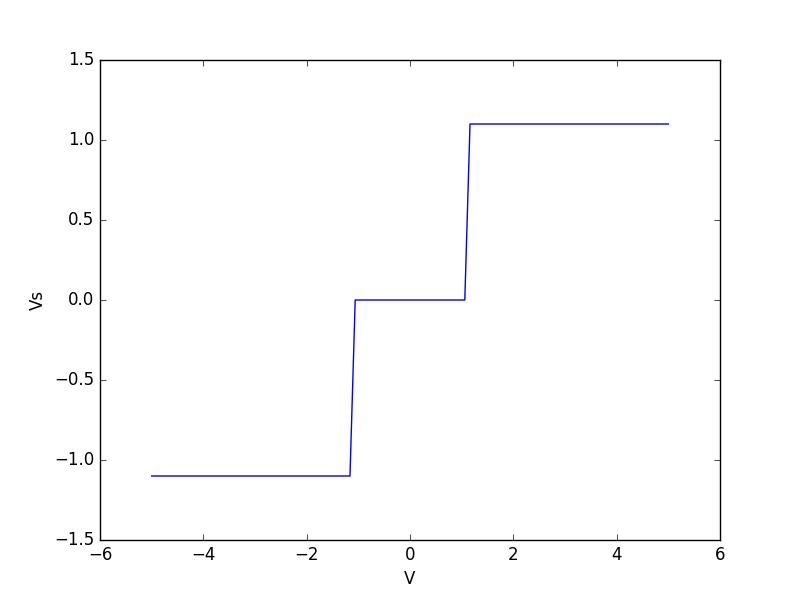
\includegraphics[width=0.8\textwidth]{figs/rel3/ex6.png}
    \caption{Curva da característica de transferência do sistema do problema 6}
\end{figure}

\section{Exercício 7}

Utilizando o modelo de queda de tensão constante aplicado ao diodo Zener e
analisando de forma análoga ao circuito do problema 6,

% TODO Add image for the direct wave circuit.

\begin{equation}
    v_s(t) =
    \begin{cases}
        V_Z & \forall\ V > V_Z \\
        0, & \text{caso contrário}
    \end{cases}
\end{equation}

% TODO Add image for the inverse wave circuit.

\begin{equation}
    v_s(t) =
    \begin{cases}
        -V_D & \forall\ V < V_D \\
        0, & \text{caso contrário}
    \end{cases}
\end{equation}

Sendo assim, a curva da característica de transferência do circuito pode ser desenhada
e encontra-se na figura Z.
\begin{figure}
    \centering
    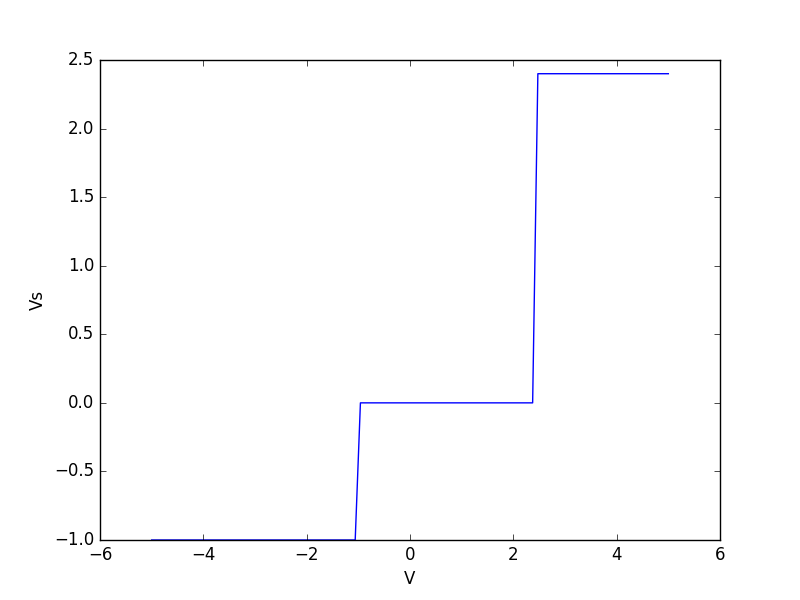
\includegraphics[width=0.8\textwidth]{figs/rel3/ex7.png}
    \caption{Curva da característica de transferência do sistema do problema 7}
\end{figure}

\section{Exercício 8}

Por analogia ao problema 6, a curva de saída deste problema pode ser obtida
intuitivamente e é visível na figura W.

\begin{figure}
    \centering
    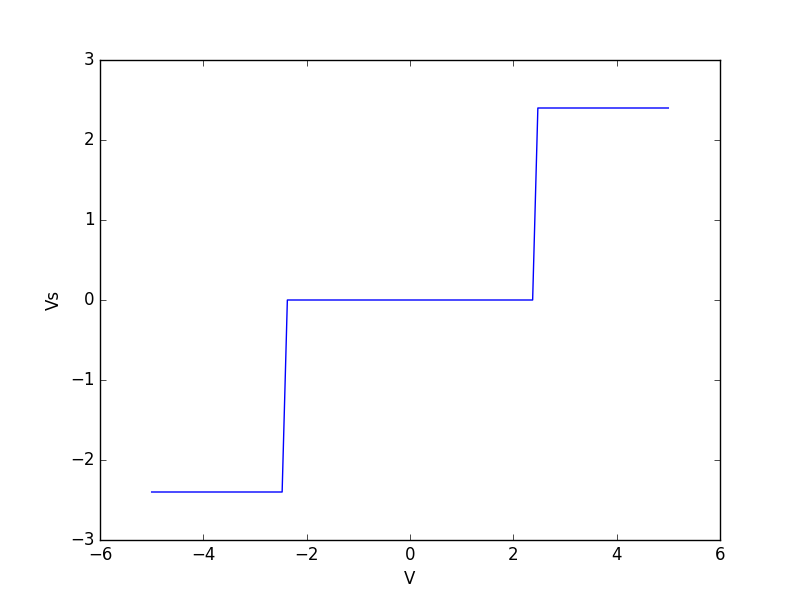
\includegraphics[width=0.8\textwidth]{figs/rel3/ex8.png}
    \caption{Curva da característica de transferência do sistema do problema 8}
\end{figure}

\section{Exercício 9}

O plágio é considerado um roubo, por ser a apropriação de uma propriedade intelectual.
No caso, se for desejado utilizar o conteúdo intelectual produzido por um terceiro,
devemos citá-lo de maneira adequada. Desta forma, estamos dando crédito ao real dono
daquela produção e estaremos contribuindo com o desenvolvimento científico. A falta de
uma citação implica que nós seríamos os autores daquele texto.

\section{Exercício 10}

A \textit{ABNT} (Associação Brasileira de Normas Técnicas) é uma sociedade privada e
sem fins lucrativos que visa normatizar a produção técnica e intelectual no Brasil por
meio de normas técnicas. No caso, se queremos lançar um produto ou publicar um artigo
neste país, devemos seguir um padrão determinados por comitês especializados pela ABNT
para que haja um denominador comum e que os projetos e os projetistas possam dialogar
entre si.

\section{Referência Bibliográfica}

\begin{itemize}
    \item SCHROEN, Walter H. "Characteristics of High-Current, High-Voltage Shockley
    Diode." IEEE Transactions on Electron Devices, Vol. ED-17, No. 9. September 1970.
    \item Datasheet do 1N4007 da Fairchild Instruments. Acesso em 18 de Setembro de
    2017.
    \item Notas de aula do professor Geovanny.
\end{itemize}

\end{document}
